\documentclass[12pt]{extarticle}
\usepackage{amsmath, amsthm, latexsym, tikz, graphicx, listings, microtype, mathtools, soul, color, fancyhdr}
\usepackage[margin=1in]{geometry}

\newenvironment{myindentpar}[1]%
 {\begin{list}{}%
         {\setlength{\leftmargin}{#1}}%
         \item[]%
 }
 {\end{list}}
 
\DeclarePairedDelimiter\abs{\lvert}{\rvert}%
\DeclarePairedDelimiter\norm{\lVert}{\rVert}%

% Swap the definition of \abs* and \norm*, so that \abs
% and \norm resizes the size of the brackets, and the 
% starred version does not.
\makeatletter
\let\oldabs\abs
\def\abs{\@ifstar{\oldabs}{\oldabs*}}
%
\let\oldnorm\norm
\def\norm{\@ifstar{\oldnorm}{\oldnorm*}}
\makeatother

\definecolor{lightgray}{gray}{0.65}
\definecolor{pinegreen}{RGB}{1, 171, 161}
\definecolor{lightblue}{RGB}{135, 206, 250}
\definecolor{dkgreen}{rgb}{0,0.6,0}
\definecolor{gray}{rgb}{0.5,0.5,0.5}
\definecolor{mauve}{rgb}{0.58,0,0.82}
\definecolor{darkblue}{rgb}{0.0,0.0,0.6}
\definecolor{cyan}{rgb}{0.0,0.6,0.6}

\newcommand*{\Value}{\frac{1}{2}x^2}%
\newcommand{\hlc}[2][yellow]{ {\sethlcolor{#1} \hl{#2}} }


% /*--------------------------------------------------------------*/
%   Changing the values here sets the due date for the assignment!
% /*--------------------------------------------------------------*/
\newcommand{\duedate}{XX/XX/XX }
\newcommand{\semester}{SEMESTER}

\lstset{frame=tb,
  language=C++,
  breaklines=true,
  showstringspaces=false,
  columns=flexible,
  numbers=none,
  tabsize=3,
  escapeinside={(*@}{@*)}
  %,
  %commentstyle=\color{dkgreen},
  %stringstyle=\color{mauve}
}
\pagestyle{fancy}
\fancyhf{}
\renewcommand{\headrulewidth}{0pt}
\lhead{\color{lightgray} CSCE-313}
\rhead{\color{lightgray} \semester}
\rfoot{\thepage}
\pagenumbering{arabic}

\definecolor{codegray}{gray}{0.9}
\newcommand{\code}[1]{\colorbox{codegray}{\texttt{#1}}}

\begin{document}


\begin{center}
    \underline{{\large Machine Problem 5: The UNIX Shell \  }(Due: \duedate)}  \\
\end{center}

\ \\
{\large \underline{Introduction}:}

\begin{myindentpar}{5mm}

Most useful interaction with a UNIX system occurs through the shell.  Using a series of easy to remember and simple commands, one can navigate the UNIX file system and issue commands to perform a wide variety of tasks.  Even though it may appear simple, the shell encapsulates many significant components of the operating system.  

\end{myindentpar}

\ \\
{\large \underline{Basic Shell Features}:}

\begin{myindentpar}{5mm}

\noindent
\textbf{Environment}

\ \\
The shell maintains many variables which allow the user to maintain settings and easily navigate the filesystem.  Two of these that are particularly important are the current working directory and the PATH.  As its name implies, the current working directory variable keeps track of the user's current directory.  The PATH variable consists of string of colon separated pathnames.  Whenever you type a name of a command, the kernel searches in the directories specified by the PATH variable starting with the leftmost directory first.  If the executable is not found in any of the specified directories, then the shell returns with an error.  One may modify the PATH at any time to add and remove directories to search for executables.  

\begin{center}
    Figure \#1: Current Directory \& PATH
\end{center}
\begin{center}
    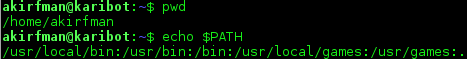
\includegraphics{environment.png}
\end{center}

\ \\
\textbf{Pipelining}

\ \\
UNIX provides a variety of useful programs for you to use (grep, ls, echo, to name a few).  Like instructions in C++, these programs tend to be quite effective at doing one specific thing (Such as grep searching text, ls printing directories, and echo printing text to the console).  However, programmers/OS users would like to accomplish large tasks consisting of many individual operations.  Doing such requires using results from previous steps in order to complete a larger problem.  The UNIX shell supports this through the pipe operation (represented by the character $\vert$).  A pipe inbetween two commands causes the standard output of one to be redirected into the standard input of another.  An example of this is provided below, using the pipe operation to search for all processes with the name "bash".  

\begin{center}
    Figure \#2: Piping Between Commands
\end{center}
\begin{center}
    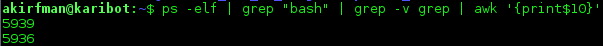
\includegraphics{pipe.png}
\end{center}

% Stuff Here (Note to self, need an advanced topic entry about dup and dup2)

\ \\
\textbf{Input/Output Redirection}

\ \\
Many times, the output of a program is not intended for immediate human consumption (if at all).  Even if someone isn't intending to look at the output of your program, it is still immensely helpful to have it print out status/logging messages during execution.  If something goes wrong, those messages can be reviewed to help pinpoint bugs.  Since it is impractical to have all messages from all system programs print out to a screen to be reviewed at a later date, sending that data to a file as it is printed is desired.  

\ \\
Other times, a program might require an extensive list of input commands.  It would be an unnecessary waste of programmer time to have to sit and type them out individually.  Instead, pre-written text in a file can be redirected to serve as the input of the program as if it were entered in the terminal window.  

\ \\
In short, the shell implements input redirection by redirecting the standard input of a program to an file opened for reading.  Similarly, output redirection is implemented by changing the standard output (and sometimes also standard error) to point to a file opened for writing.  

\begin{center}
    Figure \#3: Input/Output Redirection
\end{center}
\begin{center}
    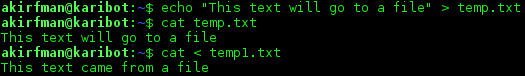
\includegraphics{redirection.png}
\end{center}

%Similar to pipes, the shell allows you to redirect the input to and output of a 
% Stuff Here (Note to self, need advanced topic about some simpler elements of file descriptors)

%\ \\
%\textbf{Modifiable Prompt}

%\ \\
%\textbf{Write paragraph here}

%\begin{center}
%    Figure \#4: PS1 Variable
%\end{center}
%\begin{center}
%    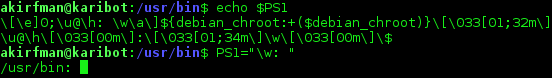
\includegraphics{ps1.png}
%\end{center}

%The prompt of the shell serves as a quick reference while you operate your computer.  Command line interfaces are inherrently low in graphic information content.  

%It would be dfficult to remember wi


\end{myindentpar}


\newpage
\noindent
{\large \underline{Assignment}:}

\begin{myindentpar}{5mm}

\vspace{-2mm}
\ \\
For this assignment, you are to design a simple shell which implements a subset of the functionality of the Bourne Again Shell (Bash).  The requirements for your shell are as follows:

\begin{itemize}
    \setlength\itemsep{-0.1em}

    \item Continually prompt for textual user input on a command line.
    \item Parse user input according the provided grammar (see below)
    \item When a user enters a well formed command, execute it in the same way as a shell.  You must use the commands fork and exec to accomplish this.  You may NOT use the C++ system() command.  
    \item Allow users to pipe the standard output from one command to the input of another an arbitrary number of times.  
    \item Support input redirection from a file and output redirection to a file.  
    \item Allow users to specify whether the process will run in the background or foreground using an '\&'.  Backgrounding processes should not result in the creation of zombie processes.  (Commands to run in the foreground do not have an '\&', and commands that run in the background do)
    \item Allow your program to take an option "-t" which will run your shell the same way, just without a prompt.  
    \item (Bonus) Allow users to specify a custom prompt which supports printing the current directory, username, current date, and current time.  

\end{itemize}

\begin{center}
    Figure \#4: Simple Shell Grammar
\end{center}
\begin{lstlisting}[frame=single]
(*@valid\_string = unix\_command PIPE unix\_command $\vert \vert$ unix\_command REDIRECTION@*)
              (*@filename $\vert \vert$ unix\_command AMP $\vert \vert$ unix\_command $\vert \vert$ special\_command@*)

(*@unix\_command = command\_name PIPE command\_name ARGS@*)

(*@special\_command = cd DIRECTORY $\vert \vert$ exit@*)

(*@command\_name = any valid executable/interpreted file name@*)

(*@AMP = \&@*)

(*@ARG = string @*)

(*@ARGS = ARG ARGS $\vert \vert$ ARG@*)

(*@DIRECTORY = absolute path $\vert \vert$ relative path@*)

(*@PIPE = $\vert$@*)

(*@REDIRECTION = $<$ $\vert \vert$ $>$@*)
\end{lstlisting}

\end{myindentpar}

\newpage
\noindent
{\large \underline{Advanced Concepts}:} 

\begin{myindentpar}{5mm}

    \vspace{3mm}
    \noindent
    \textbf{File Pathnames}
    
    \ \\
    The UNIX filesystem is organized as a giant tree.  Leaf nodes are files, and non-leaf nodes are directories which either contain files or other directories.  The highest node in the tree is root, denoted by a forward slash (/).  All other files/directories in the system are child nodes of the root node.  
    
    \ \\
    Filenames in a UNIX system are specified by a pathname (such as \code{/bin/bash} stating that the file bash is inside the directory bin which is inside of root).  Pathnames are provided either as absolute pathnames, which are given relative to the root of the filesystem (Ex: \code{/usr/bin/env}), or as relative, which are specified relative to the current working directory (\code{../../andrew/homework/CSCE\_315}).  
    
    \ \\
    Side note: UNIX contains two special paths present in each directory.  A single dot stands for the current directory, and two dots stands for the parent directory.  To see these, type the command ls -l into a shell.  
    
    \ \\
    \textbf{Process Address Space}
    
    \ \\
    The address space of a process is usually divided up into 4 regions, stack segment, dynamic data, static data, and text segment (See Figure \#4).  
    
    \ \\
    All code pertaining to the execution of the program is contained in the text segment.  Program data is stored in two sections depending on the type.  Static data (global variables and constants) is defined before the execution of the program.  As a result, this segment is of a fixed size which can be allocated on loading.  Dynamic data contains all data allocated to the process through calls to malloc/new.  Since this changes continually throughout the process's life cycle, this section of the address space grows towards higher addresses and shrinks back towards lower addresses.  Finally, the stack contains data pertaining to function calls.  As with the dynamic data segment, the stack must grow and shrink with the execution of a process.  Therefore, the stack grows downwards from high addresses towards lower ones and shrinks back to high addresses.  

\end{myindentpar}

\newpage
\begin{center}
    Figure \#4: Simple Address Space
\end{center}
\begin{center}
    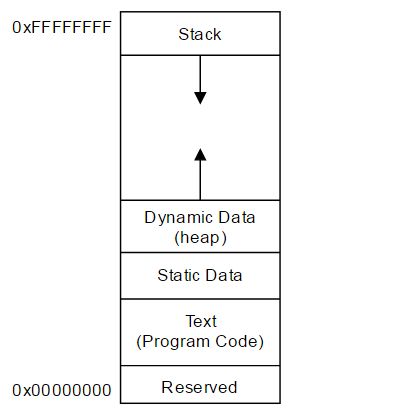
\includegraphics{memory_map.png}
\end{center}


\begin{myindentpar}{5mm}
    
    \ \\
    \textbf{fork()};
    
    \ \\
    When the operating system is initialized, three processes are created.  The first, known as the swapper (process id 0), serves as the scheduler for jobs on the system.  The second, known as init (process id 1), sets up many processes and services across the system.  After it performs its initial tasks, init becomes a looping call to wait() which reclaims the state of orphaned processes.  The third, known as the pagedaemon (process id 2), is responsible for memory management.  
    
    \ \\
    Other than these three processes started by the operating system, every other process in the system is brought to life through a call to the \code{fork()} system call.  A process calling fork is copied by the kernel.  At this point, the process that called fork is known as the parent, and the newly created process is known as the child since the parent process caused the child to be created.  The newly created process is essentially exactly the same as the child, even having the exact same variables and open files.  Fork is unique in that it is called once by the parent process and returns twice (to the parent and child separately).  To the parent, fork returns the process id (PID) of the newly created child.  To the child, fork returns 0.  If the call fails entirely, -1 is returned to the parent, and no child is created.  For more information about fork, see its manpage by calling \code{man 2 fork}.  
    
    \ \\
    Copying the entire context of a process could take quite a long time, especially if the parent process contains a large amount of data.  Instead, modern kernels perform an action called copy-on-write.  When the fork call returns, both processes point to the same regions in memory.  As soon as either process wants to write data anywhere in the address space, the kernel creates a new page in memory for that process.  Therefore, both processes use essentially all of the same memory regions initially, and they slowly diverge as time progresses.  
    
    \ \\
    A pseudocode description of the actual fork algorithm is provided below (Bach).  
    
    
\ \\
\begin{lstlisting}[frame=single]
(*@algorithm fork@*)
(*@input:@*)  (*@none@*)
(*@output: to parent proces, child PID number@*)
        (*@to child process. 0@*)
{
    (*@check for available kernel resources;@*)
    (*@get free proc table slot and unique PID number;@*)
    (*@check that user not running too many processes;@*)
    (*@mark child state as "being created";@*)
    (*@copy data from parent proc tabgle slot to new child slot;@*)
    (*@increment counts on current directory inode and changed root (if applicable);@*)
    (*@increment open file counts in file table;@*)
    (*@make copy of parent context (PCB, text, data, stack) in memory);@*)
    (*@push dummy system level context layer onto child system level context;@*)
        (*@dummy context contains data allowing child process to recognize@*)
        (*@itself, and start running from here when scheduled@*)
    (*@if(executing process is parent process)@*)
    {
        (*@change child state to "ready to run";@*)
        (*@return(child ID);@*)
    }
    (*@else@*)
    {
        (*@initialize PCB timing fields;@*)
        (*@return(0);@*)
    }

}
\end{lstlisting}
    
    \newpage
    \noindent
    \textbf{The Six Exec Functions}
    
    \ \\
    After executing \code{fork()}, you are left with two identical processes.  This isn't usually particularly useful unless you specifically need two exact copies of a process.  Instead, UNIX provides a function, known as exec, which allows you to change a process's address space in order to run an entirely new program.  Running an exec command deletes the existing text, data, and stack segments of the existing process and replaces them with with those of a new program.  The algorithm for exec is presented below (Bach 218).  
    
\ \\
\begin{lstlisting}[frame=single]
(*@algorithm exec@*)
(*@input: @*)  (*@(1) file name@*)
        (*@ (2) parameter list@*)
        (*@ (3) environment variables list@*)
(*@output: none@*)
{
    (*@get file inode (algorithm namei);@*)
    (*@very file is executable and user has permission to execute;@*)
    (*@read file headers, check that it is a load module;@*)
    (*@copy exec parameters from old address space to system space;@*)
    (*@for(every region attached to process)@*)
    {
        (*@detach all old regions (algorithm detach);@*)
    }
    (*@for(every region specified in load module)@*)
    {
        (*@allocate new regions (algorithm allocreg);@*)
        (*@attach the regions (algorithm attachreg);@*)
        (*@load region into memory if appropriate (algorithm loadreg);@*)
    }
    (*@copy exec parameters into new user stack region;@*)
    (*@special processing for setuid programs, tracing;@*)
    (*@initialize user register save area for return to user mode;@*)
    (*@release inode of file (algorithm iput)@*)
}
\end{lstlisting}

    \ \\
    In UNIX systems, there is only one algorithm for exec, but the system call interface provides a total of six different variations of the exec function which differ only on how they handle input arguments.  This means that only one system call (usually \code{execve()}) is actually required to be implemented.  The other functions are stubs with perform necessary preparations and then eventually call execve.  Short descriptions of each version along with short examples are provided below (Setvens 207-209).  

    \begin{center}
        Exec Functions \& Examples
    \end{center}
\begin{lstlisting}[frame=single]
#include<unistd.h>

1. int execl(const char *pathname, const char *arg0, ... (*@/* (char *) 0 */ @*));

    (*@Example: @*)
    execl("/bin/bash", "bash", "-c", "echo \"Hello World!\"", NULL);

2. int execv(const char *pathname, char *const argv[]);

    (*@Example: @*)
    argv = {"/bin/bash", "-c", "echo \"Hello World\""}
    execv("/bin/bash", &argv);


(*@The following exec commands take an environment array (envp) in addition @*)
(*@to the other arguments.  This can be used to define a custom environment @*)
(*@for the process.  Otherwise, uses parent's environment.  @*)

3. int execle(const char *pathname, const char *arg0, ... (*@/* (char *) 0 */ @*), 
    char *const envp[]);

4. int execve(const char *pathname, char *const argv[], char *const envp[]);


(*@Exec commands ending in a p use the PATH environ variable in order to find@*)
(*@the executable file.  An error is thrown if the file is not in a directory@*)
(*@specified by PATH.  @*)

5. int execlp(const char* filename, const char *arg0, ... (*@/* (char *) 0 */ @*));

6. int execvp(const char *filename, char *const argv[]);


(*@All return -1 on error and do not return when successful@*)
\end{lstlisting}

    \ \\
    \textbf{Zombie Processes}
    
    \ \\
    The commands, \code{wait()} and \code{waitpid()} are critical for proper process creation.  Without them, there would be no way for the parent to recover any data about any of its child processes.  Depending on the success or failure of one of it's children, the parent may need to perform actions in a variety of different ways.  
    
    \ \\
    Once a process dies, the kernel cannot assume that the parent process will call wait immediately.  It only knows that it has to leave the option to call wait until the parent does so.  Consequently, the kernel must maintain a limited number of data elements from the finished/terminated process for the parent to read.  In order to do so without wasting unnecessary space, the kernel reclaims all portions of the process not pertaining to what it needs to deliver to the parent.  The remaining shell of the process is known as a zombie.  
    
    \ \\
    In the case of bad programming practice, a parent process may never call wait before it terminates.  When the parent terminates, all child processes that it spawned are orphaned.  Obviously, it would be disastrous to simply leave these zombie processes to never be reclaimed.  Eventually, so much system memory would be used up that a complete system restart would be required.  
    
    \ \\
    Instead, the kernel designates a special process to become the foster parent of all orphaned processes.  On all Linux/UNIX systems, this process is init (process 1).  After init performs all required tasks at system startup, it becomes a while loop containing a wait statement.  It constantly reaps processes left behind by their parents and prevents the formation of zombies.  
    
\end{myindentpar}

\newpage
\noindent
{\large \underline{UNIX man Pages}:}

\begin{myindentpar}{5mm}

    One incredibly useful feature of UNIX operating systems that many new developers do not know about is the built in manual system.  Using the command 'man', you can access information about most aspects of the operating system from general commands all the way to system call APIs.  
    
    \ \\
    The structure of man pages in UNIX are organized into sections by number follows (Wikimedia Foundation):
    \begin{enumerate}
        \setlength\itemsep{-0.1em}
        
        \item General Commands
        \item System Calls
        \item Library Functions (Specifically, the C standard library)
        \item Special Files
        \item File Formats
        \item Games
        \item Miscellanea
        \item System Administration
        
    \end{enumerate}
    
    \ \\
    You may (or may not, that's fine too) find the following manual pages useful when creating this assignment.  Each one of these lines can be executed as a valid shell command to open a particular manual page.  Note, the number indicates the manual section that that function resides.  
    
    \begin{itemize}
        \setlength\itemsep{-0.1em}
    
        \item \code{man 3 exec}
        \item \code{man 2 fork}
        \item \code{man 2 chdir}
        \item \code{man 2 pipe}
        \item \code{man 2 dup}
        \item \code{man 2 wait} (Hint: Pay particular attention to waitpid and the option ONOHANG)
     
    \end{itemize}

\end{myindentpar}

\newpage
\noindent
{\large \underline{Bibliography}:}

\ \\
{[} 1 {]} \hspace{1.2mm} Bach, Maurice J. \textit{The Design of the UNIX Operating System}. Englewood Cliffs, NJ:
\hspace*{1cm} Prentice-Hall, 1986. Print.

\ \\
{[} 2 {]} \hspace{1.2mm} Stevens, W. Richard. \textit{Advanced Programming in the UNIX Environment}. Reading,
\hspace*{1cm} MA: Addison-Wesley Pub., 1992. Print.

\ \\
{[} 3 {]} \hspace{1.2mm} "Man Page." Wikipedia. Wikimedia Foundation, n.d. Web. 18 May 2016.


\end{document}